\documentclass[14pt, a4paper]{article}

\usepackage[utf8]{inputenc}
\usepackage[T2A]{fontenc}

\usepackage{graphicx}
\graphicspath{ {images/} }

\tolerance 1414
\hbadness 1414
\emergencystretch 1.5em
\hfuzz 0.3pt        % размер максимального переполнения без warning'a
\widowpenalty=10000 % запрещает одиночную строку абзаца в начале страницы 
\vfuzz \hfuzz
\raggedbottom       % если на странице мало содержимого, добавить пустое место в конце, а не в середине страницы

\title{ЛАБОРАТОРНАЯ РАБОТА №2
Неразветвленные цепи синусоидального тока
}
\author{Новоженов П.А. ЭН-26}
\date{}

\begin{document}

    \maketitle

    \thispagestyle{empty}

    \clearpage

    \section*{Цель работы}
        Практическое ознакомление с установившимися режимами в
        последовательных RL-, RC- и RLC-цепях синусоидального тока.

    
    \section*{Задание 1. Расчет индуктивного сопротивления}

        % Скрин таблицы

        $$L = 85 mH \ \ \ C = 160 \ \mu F$$
        $$X_L = 2\pi f L$$
        $$X_{L30} = 2\cdot \pi \cdot 30 \cdot 85 \cdot 10^{-3} = 16$$
        $$X_{L40} = 2\cdot \pi \cdot 40 \cdot 85 \cdot 10^{-3} = 21$$
        $$X_{L50} = 2\cdot \pi \cdot 50 \cdot 85 \cdot 10^{-3} = 27$$
        $$X_{L60} = 2\cdot \pi \cdot 60 \cdot 85 \cdot 10^{-3} = 32$$
        $$X_{L80} = 2\cdot \pi \cdot 80 \cdot 85 \cdot 10^{-3} = 43$$
        $$X_{L100} = 2\cdot \pi \cdot 100 \cdot 85 \cdot 10^{-3} = 53$$
        $$X_{L120} = 2\cdot \pi \cdot 120 \cdot 85 \cdot 10^{-3} = 64$$
 
        $$X_{C} = \frac{1}{2\pi f C}$$ 
        $$X_{C30} = \frac{1}{2\pi \cdot 30 \cdot 160 \cdot 10^{-6}} =  33$$  
        $$X_{C40} = \frac{1}{2\pi \cdot 40 \cdot 160 \cdot 10^{-6}} = 24$$
        $$X_{C50} = \frac{1}{2\pi \cdot 50 \cdot 160 \cdot 10^{-6}} = 19$$
        $$X_{C60} = \frac{1}{2\pi \cdot 60 \cdot 160 \cdot 10^{-6}} = 16$$
        $$X_{C80} = \frac{1}{2\pi \cdot 80 \cdot 160 \cdot 10^{-6}} = 12$$
        $$X_{C100} = \frac{1}{2\pi \cdot 100 \cdot 160 \cdot 10^{-6}} = 9$$
        $$X_{C120} = \frac{1}{2\pi \cdot 120 \cdot 160 \cdot 10^{-6}} = 8$$

        {
            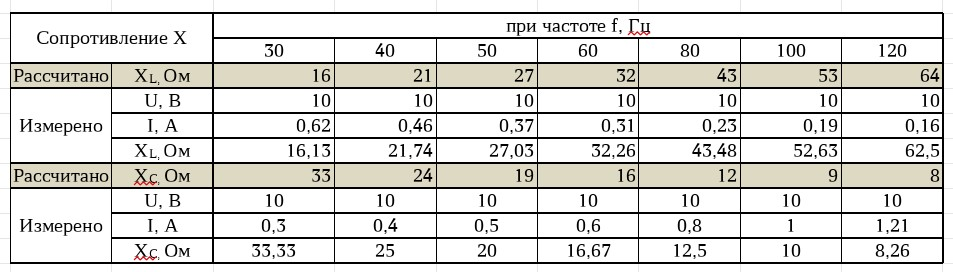
\includegraphics[width=0.8\textwidth]{Table.jpg}
            \centering
        }

        {
            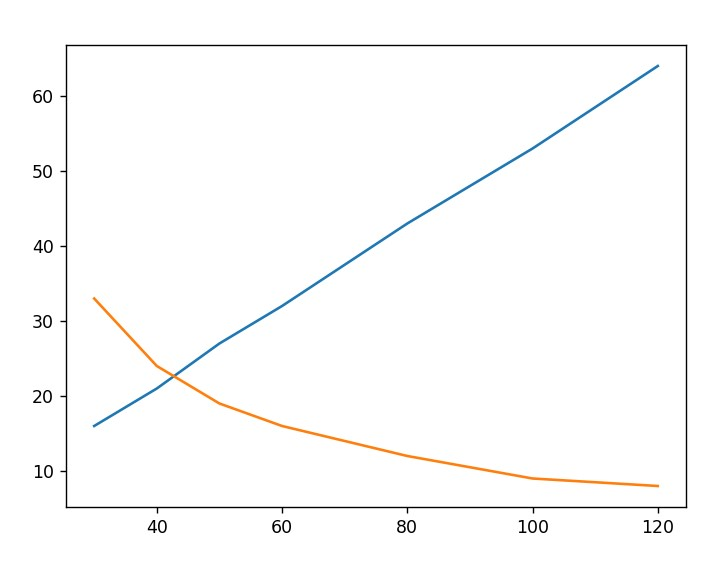
\includegraphics[width=0.8\textwidth]{graph1.jpg}
            \centering
        }

    \section*{Задание 2. Настройка схемы}

        {
            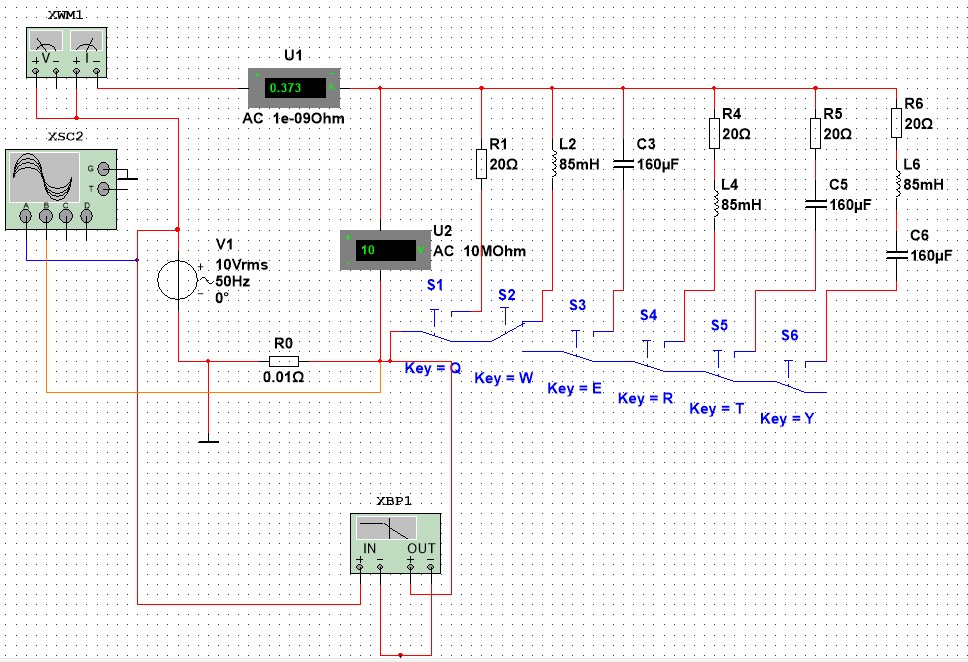
\includegraphics[width=0.8\textwidth]{Design.jpg}
            \centering
        }

    \section*{Задание 3. Измерения в цепях с одним элементом}

        $$ I = \frac{U}{R_1} = \frac{9.995}{20} = 0.49975 \approx 0.5 \ A $$

        {
            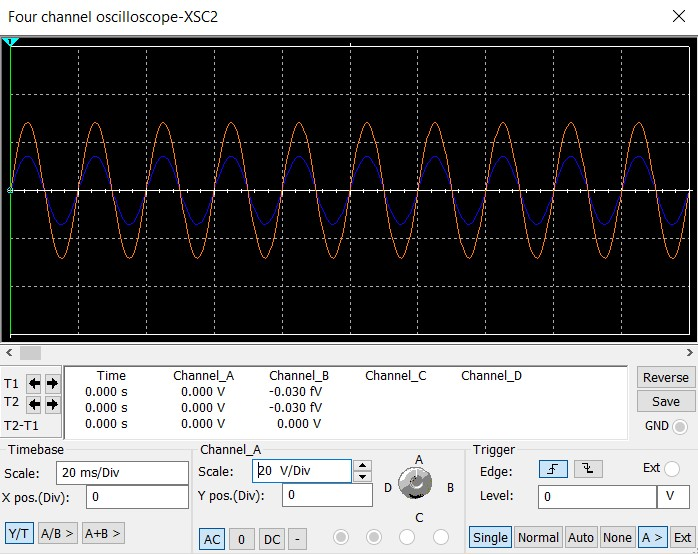
\includegraphics[width=0.8\textwidth]{O1.jpg}
            \centering
        }

        Сдвиг фаз между напряжением и током равен нулю.

        {
            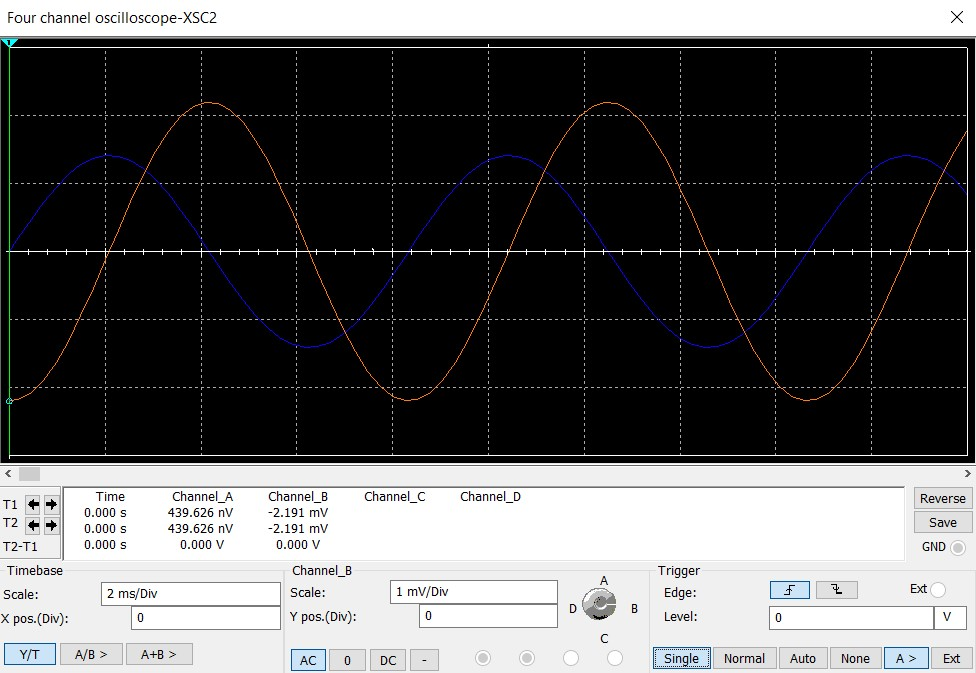
\includegraphics[width=0.8\textwidth]{O2.jpg}
            \centering
        }

        Видим, что ток отстает от напряжения на $\frac{\pi}2$.


        {
            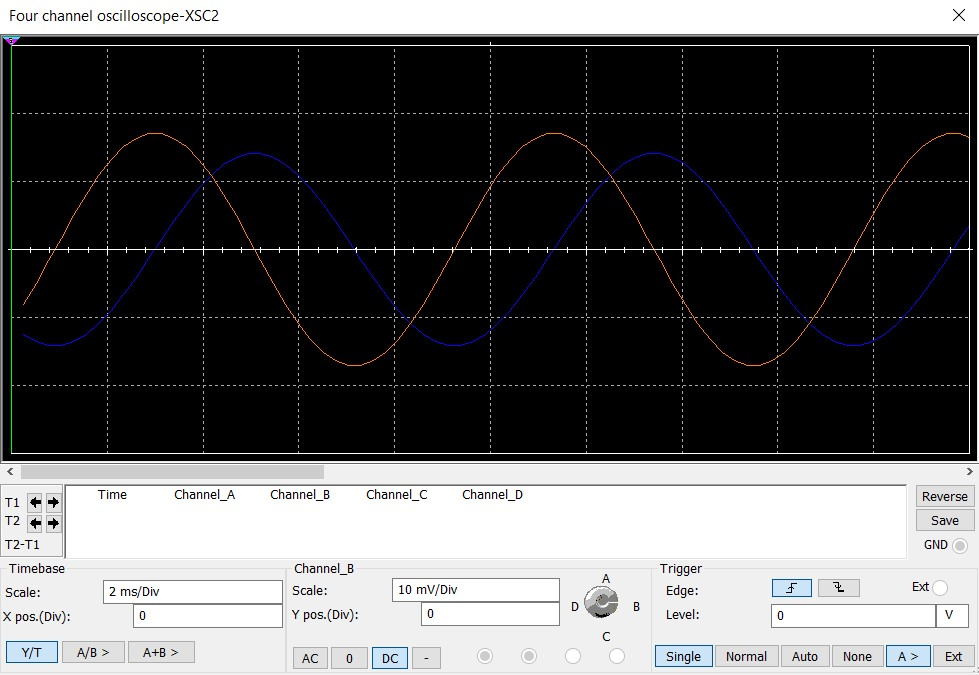
\includegraphics[width=0.8\textwidth]{O3.jpg}
            \centering
        }

        Видим, что ток опережает по фазе напряжение на $\frac{\pi}2$.

        {
            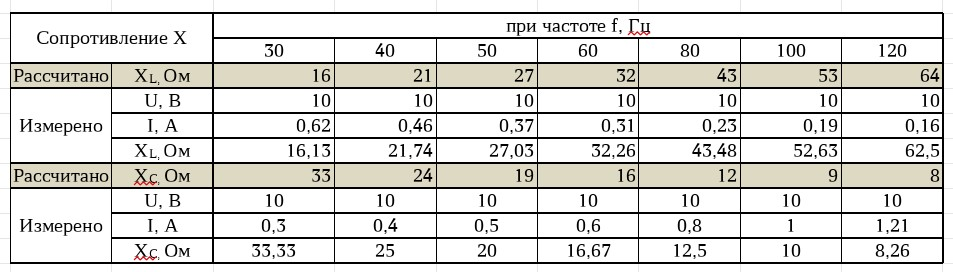
\includegraphics[width=0.8\textwidth]{Table.jpg}
            \centering
        }

    \section*{Задание 4. Измерения в RL, RC и RLC ветвях}

        \subsection*{Для цепи $R_4L_4$.}
        {
            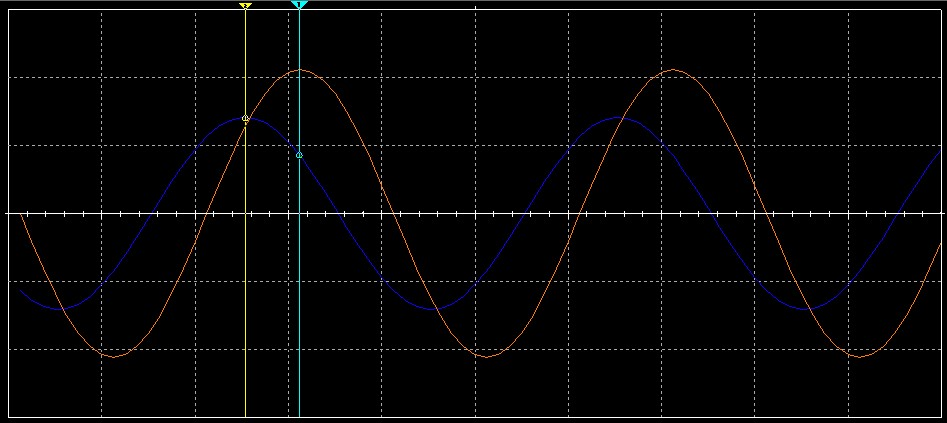
\includegraphics[width=0.8\textwidth]{RL_osc.jpg}
            \centering
        }

        Заметим, что ток отстает от напряжения на величину $\varphi_4$:
        $$\varphi_4 = \arctan(\frac{X_4}{R_4}) \approx 53^\circ$$

        \subsection*{Для цепи $R_5C_5$.}

        {
            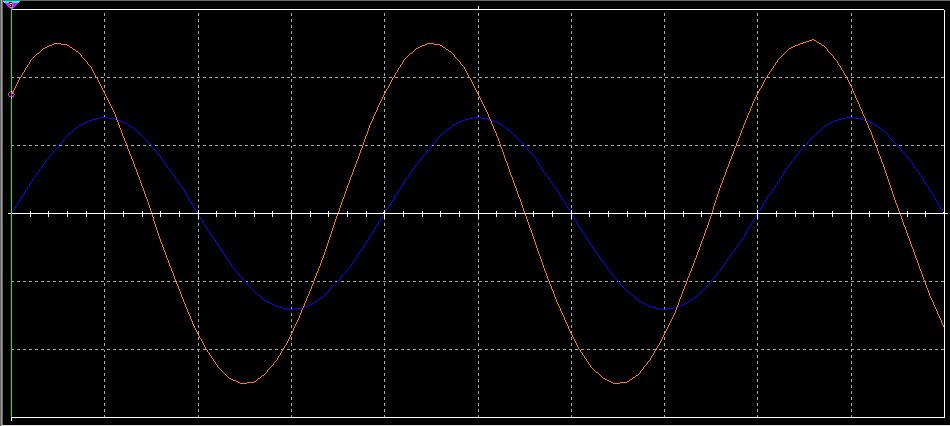
\includegraphics[width=0.8\textwidth]{RC_osc.jpg}
            \centering
        }

        Заметим, что ток опережает напряжение на величину $\varphi_5$:
        $$\varphi_5 = \arctan(\frac{X_5}{R_5}) \approx 44^\circ$$

        \subsection*{Для цепи $R_6C_6L_6$.}

        {
            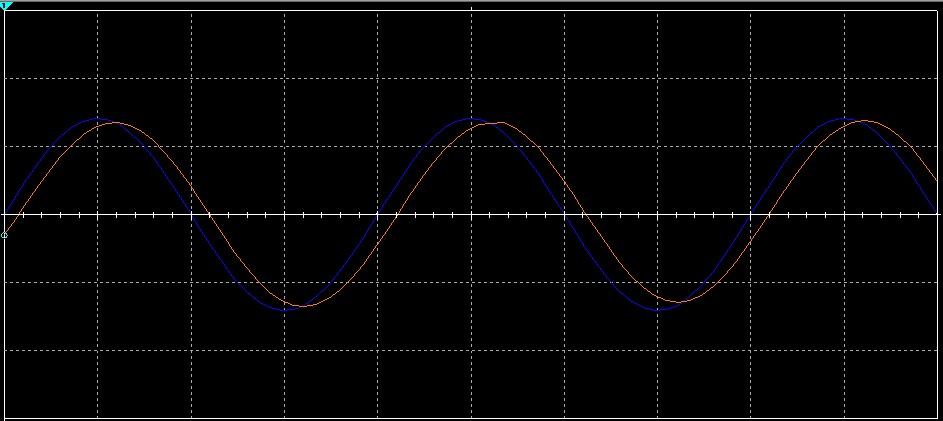
\includegraphics[width=0.8\textwidth]{RCL_osc.jpg}
            \centering
        }

        При частоте 50 Гц ток отстает от напряжения. Изменим частоту до 20 Гц и ток начнет опережать напряжение.

        {
            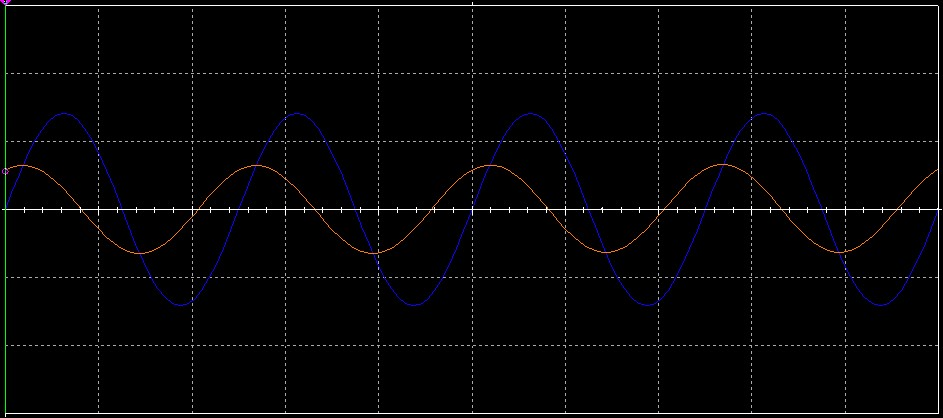
\includegraphics[width=0.8\textwidth]{RCL_osc20.jpg}
            \centering
        }

        {
            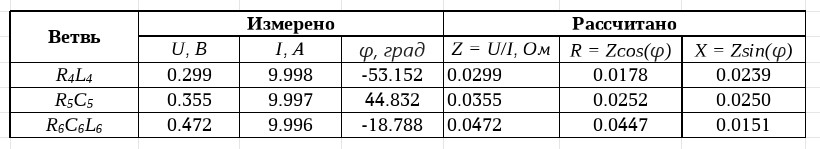
\includegraphics[width=0.8\textwidth]{Table2.jpg}
            \centering
        }
        
    \section*{Вывод}
        В ходе данной работы я на практике ознакомился с установившимися режимами в последовательных RL, RC, RLC цепях синусоидального тока.





        
\end{document}